\chapter{ಲೇಖನಿ – ಚಿತ್ರ ಬಿಡಿಸುವುದು}
ಈವರೆಗೂ ಸ್ಪ್ರಯ್ಟ್ ಗೆ ಆಜ್ಞೆಗಳನ್ನಿತ್ತು ಅದನ್ನು ಅತ್ತಿತ್ತ ಓಡಾಡಿಸಿದೆವು.  ಕಂಪ್ಯೂಟರ್, ಆಜ್ಞೆಗಳನ್ನು  ಅತಿ ವೇಗವಾಗಿ ಮಾಡಿಬಿಡುತ್ತದೆ.  ಆದ್ದರಿಂದ ಸ್ಪ್ರಯ್ಟ್ ಓಡಡಿದ ಹಾದಿ ತಿಳಿಯುವುದ್ ಕಷ್ಟ ವಾಗುತ್ತದೆ.  ಆಜ್ಞೆಗಳನ್ನು ಹಂತ ಹಂತವಾಗಿ ಮಾಡುವುದನ್ನು ನೋಡಬೇಕಾದರೆ, ಕಂಪ್ಯೂಟರನ್ನು ಕಾಯ್ದಿರಿಸಿವುದನ್ನೂ ನೋಡಿದ್ದೇವೆ. ಹಾಗೆ ಕಾಯಿಸುವುದು ಬೇಡವೆಂದರೆ, ಸ್ಪ್ರಯ್ಟ್ ಓಡಾಡುವಾಗ ಒಂದು ಲೇಖನಿಯನ್ನು (\textenglish{pen})ಹಿಡಿದು ಓಡಡಿದರೆ, ಅದರ ಹಾದಿ ನಮಗೆ ತಿಳಿಯುತ್ತದಲ್ಲವೇ? 

ಸ್ಕ್ರಾಚ್ನಲ್ಲಿ ಲೇಖನಿಗೆಂದೇ ಆಜ್ಞೆಗಳ ಒಂದು ಗುಂಪು ಇದೆ. ಇದರಲ್ಲಿನ ಆಜ್ಞೆಗಳನ್ನು ಹೇಗೆ ಉಪಯೋಗಿಸಿಕೊಳ್ಳುವುದೆಂದು ಈಗ ತಿಳಿಯೋಣ. 
\section{ಲೇಖನಿಯುಕ್ತ - ಮುಕ್ತ}
ಮೊದಲಿಗೆ ಹಸಿರು ಬಣ್ಣದ "ಲೇಖನಿ" ಗುಂಪನ್ನು ಒತ್ತಿ ಅದರಲ್ಲಿನ ಆಜ್ಞೆಗಳನ್ನು ಗಮನಿಸಿ.  ಇವುಗಳ್ಳಲ್ಲಿ ಲೇಖನಿಯುಕ್ತ ಎಂಬ  ಆಜ್ಞೆ ಬಳಸಿ ಸ್ಪ್ರಯ್ಟ್ ಅನ್ನು ಲೇಖನಿಯುಕ್ತ ಮಾಡಬಹುದು. ಹಾಗೆ ಮಾಡಿದ ನಂತರ ಸ್ಪ್ರಯ್ಟ್ ಎಲ್ಲೆಲ್ಲಿ ನಡೆದಾಡುವುದೊ ಅಲ್ಲೆಲ್ಲಾ ಗೆರೆಗಳು ಮೂಡಿಬರುವುದನ್ನು ಕಾಣಬಹುದು - ಒಂದು ರೀತಿಯಲ್ಲಿ ಬೆಕ್ಕಿಗೆ ಗೀಚಾಡಲು ಅನುಮತಿ ನೀಡಿದಂತೆ.  ಅಷ್ಟಕ್ಕೂ ಇದು "\textenglish{SCRATCH}" ಸ್ಕ್ರಾಚ್ ಅಲ್ಲವೇ? 

ಈಗಾಗಲೇ ಉಪಯೋಗಿಸಿದ ಪ್ರೋಗ್ರಾಮನ್ನೆ ಮತ್ತೆ ಬಳಸೋಣ.  ಚಿತ್ರ \ref{program3} ನಲ್ಲಿರುವ ಪ್ರೋಗ್ರಾಂ ಸ್ಪ್ರಯ್ಟ್ ಅನ್ನು ಚೌಕಾಕಾರವಾಗಿ ಒಡಾಡಿಸುತ್ತದ,  ಆದರೆ ಚೌಕ ಮೂಡುವುದಿಲ್ಲವಷ್ಟೆ. ಅದೇ ಪ್ರೋಗ್ರಾಮ್ಮಿಗೆ ಲೇಖನಿಯುಕ್ತ ಮಾಡಿ ನೋಡೋಣ.

\begin{figure}[h]
\begin{center}
\begin{multicols}{2}
\begin{Scratch}[1]
\beginbox{}
\scbox{ಲೇಖನಿಯುಕ್ತ}{pen}
\scbox{\cb[w]{100} ಹೆಜ್ಜೆ ಮುಂದೆ ಹೋಗು}{motion}
\turnbox{1}{90}{ಡಿಗ್ರಿಯಷ್ಟು ತಿರುಗು}
\scbox{\cb[w]{100} ಹೆಜ್ಜೆ ಮುಂದೆ ಹೋಗು}{motion}
\turnbox{1}{90}{ಡಿಗ್ರಿಯಷ್ಟು ತಿರುಗು}
\scbox{\cb[w]{100} ಹೆಜ್ಜೆ ಮುಂದೆ ಹೋಗು}{motion}
\turnbox{1}{90}{ಡಿಗ್ರಿಯಷ್ಟು ತಿರುಗು}
\scbox{\cb[w]{100} ಹೆಜ್ಜೆ ಮುಂದೆ ಹೋಗು}{motion}
\end{Scratch}

\begin{tikzpicture}
\node[doc] (x) (inst1){
ಒತ್ತಿದಾಗ\\
ಲೇಖನಿಯುಕ್ತ\\
100  ಹೆಜ್ಜೆ ಮುಂದೆ ಹೋಗು\\
90$‌^\circ$ ಬಲಕ್ಕೆ  ತಿರುಗು\\
100  ಹೆಜ್ಜೆ ಮುಂದೆ ಹೋಗು\\
90$‌^\circ$ ಬಲಕ್ಕೆ  ತಿರುಗು\\
100  ಹೆಜ್ಜೆ ಮುಂದೆ ಹೋಗು\\
90$‌^\circ$ ಬಲಕ್ಕೆ  ತಿರುಗು\\
100  ಹೆಜ್ಜೆ ಮುಂದೆ ಹೋಗು
};
\end{tikzpicture}

\end{multicols}

\begin{tikzpicture}
\node at (0,0)[rotate=0, opacity=0.2](s1){};
\draw[draw=blue](s1.center)--++(2cm,0)node(newcoord){};
\node at (newcoord)[rotate=-90, opacity=0.2](s2){};
\draw[draw=blue](s2.center)--++(0,-2cm)node(newcoord){};
\node at (newcoord)[rotate=-180, opacity=0.2](s3){};
\draw[draw=blue](s3.center)--++(-2cm,0cm)node(newcoord){};
\node at (newcoord)[rotate=90, opacity=0.2](s4){};
\draw[draw=blue](s4.center)--++(0,2cm)node(newcoord){};
\node at (newcoord)[rotate=90, opacity=1](s2){\Scratchy[0.2]};
\end{tikzpicture}
\end{center}
\caption{ಸ್ಪ್ರಯ್ಟ್  ಚೌಕ ಬಿಡಿಸುವುದು}
\label{pen_sqr}
\end{figure}
ಚಿತ್ರ \ref{program3} ನಲ್ಲಿರುವ ಪ್ರೋಗ್ರಾಮ್ಮನ್ನು ಮತ್ತೆ ಮೂಡಿಸಿ. ಲೇಖನಿಯುಕ್ತ ಆಜ್ಞೆಯನ್ನು ತಂದು ಚಿತ್ರ \ref{pen_sqr}ರ ಎಡಭಾಗದಲ್ಲಿರುವಂತೆ  ಜೋಡಿಸಿ.   ಪ್ರೋಗ್ರಾಂ ಅನ್ನು  ಚಲಾಯಿಸಿ (ವೇದಿಕೆಯ ಮೇಲಿನ ಹಸಿರು ಧ್ವಜವನ್ನು ಒತ್ತಿ).  ಚಿತ್ರ \ref{pen_sqr}ರ ಕೆಳಭಾಗದಲ್ಲಿ ತೋರಿಸಿರುವಂತೆ, ಥಟ್ಟನೆ ಸ್ಪ್ರಯ್ಟ್ ಚೌಕ ಮೂಡಿಸುತ್ತದೆ.

ಚಿತ್ರ \ref{pen_sqr}ನ ಬಲಭಾಗದಲ್ಲಿರುವಂತೆ  ಈ ಪ್ರೊಗ್ರಾಂ ಆನ್ನು ಪುಸ್ತಕದಲ್ಲಿ  ಸರಳವಾಗಿ ಬರೆದುಕೊಳ್ಳಬಹುದು.   ಇದರಲ್ಲಿ ಗಮನಿಸಿ, ಸ್ಪ್ರಯ್ಟ್  ತಾನು ಮೊದಲಿದ್ದ ದಿಕ್ಕಿನಲ್ಲಿ ಮುಖ ಮಾಡಿ ನಿಂತಿಲ್ಲ.  ಆದರೆ ಈಗ ಅದ್ದನ್ನು ತಿದ್ದುವುದು ಹೇಗೆ ಎಂದು ನಮಗೆ ತಿಳಿದಿದೆಯಲ್ಲವೇ?

ಬೆಕ್ಕಿನ ಕಾಲಿಗೆ ಲೇಖನಿ ಸಿಕ್ಕಿಸಿ ಬಿಟ್ಟರೆ ಗೀಚಾಡಿದಂತೆಯೇ ಸರಿ. ಆದರೆ ಅರ್ಥಪೂರ್ಣವಾದ ಚಿತ್ರಗಳನ್ನು ಮೂಡಿಸಬೇಕಾದರೆ ಆಗಾಗ್ಗೆ ಸ್ಪ್ರಯ್ಟ್ ಅನ್ನು ಲೇಖನಿಮುಕ್ತ ಮಾಡಬೇಕು.  ಇದಕ್ಕೆ ಹಸಿರು ಬಣ್ಣದ "ಲೇಖನಿ" ಗುಂಪಿನಲ್ಲಿ ಲೇಖನಿಮುಕ್ತ ಎಂಬ ಆಜ್ಞೆ ಇದೆ.  ಇದನ್ನು ಒಂದು ಉದಾಹರಣೆಯಲ್ಲಿ ಬಳಸೋಣ.  ಚಿತ್ರ \ref{pen_broken_line} ನಲ್ಲಿರುವ ಪ್ರೋಗ್ರಾಮ್ಮನ್ನು ಸ್ಕ್ರಾಚ್ನಲ್ಲಿ ಮೂಡಿಸಿ. ಈ ಪ್ರೊಗ್ರಾಂ ಏನು ಕೆಲಸ ಮಾಡಬಹುದು ಅಥವಾ ಯಾವ ಚಿತ್ರ ಮೂಡಿಸಬಹುದು ಎಂದೊಮ್ಮೆ ಯೋಚಿಸಿ.  ಈಗ ವೇದಿಕೆಯ ಮೇಲಿನ ಹಸಿರು ಧ್ವಜವನ್ನು ಒತ್ತಿ, ನಿಮ್ಮ ಅಲೋಚನೆ ಅಥವಾ ಊಹೆ ಸರಿಯಿದೆಯೇ ಎಂದು ಖಚಿತ ಪಡಿಸಿಕೊಳ್ಳಿ. 

\begin{figure}[h]
\begin{center}
\begin{multicols}{2}
\begin{Scratch}[1]
\beginbox{}
\scbox{ಲೇಖನಿಯುಕ್ತ}{pen}
\scbox{\cb[w]{100} ಹೆಜ್ಜೆ ಮುಂದೆ ಹೋಗು}{motion}
\scbox{ಲೇಖನಿಮುಕ್ತ}{pen}
\scbox{\cb[w]{100} ಹೆಜ್ಜೆ ಮುಂದೆ ಹೋಗು}{motion}
\scbox{ಲೇಖನಿಯುಕ್ತ}{pen}
\scbox{\cb[w]{100} ಹೆಜ್ಜೆ ಮುಂದೆ ಹೋಗು}{motion}
\end{Scratch}

\begin{tikzpicture}
\node[doc] (x) (inst1){
ಒತ್ತಿದಾಗ\\
ಲೇಖನಿಯುಕ್ತ\\
100  ಹೆಜ್ಜೆ ಮುಂದೆ ಹೋಗು\\
ಲೇಖನಿಮುಕ್ತ\\
100  ಹೆಜ್ಜೆ ಮುಂದೆ ಹೋಗು\\
ಲೇಖನಿಯುಕ್ತ\\
100  ಹೆಜ್ಜೆ ಮುಂದೆ ಹೋಗು
};
\end{tikzpicture}

\end{multicols}

\begin{tikzpicture}
\node at (0,0)[rotate=0, opacity=0.2](s1){};
\draw[draw=blue](s1.center)--++(2cm,0)node(newcoord){};
\node at (newcoord)[rotate=0, opacity=0.2](s2){};
\draw[draw=none](s2.center)--++(2cm,0cm)node(newcoord){};
\node at (newcoord)[rotate=-0, opacity=0.2](s3){};
\draw[draw=blue](s3.center)--++(2cm,0cm)node(newcoord){};
\node at (newcoord)[rotate=0, opacity=1](s4){\Scratchy[0.2]};
\end{tikzpicture}
\end{center}
\caption{ಸ್ಪ್ರಯ್ಟ್ ಇಂದ್ ಮುರಿದ ರೇಖೆ ಬಿಡಿಸುವುದು}
\label{pen_broken_line}
\end{figure}

ಸ್ಪ್ರಯ್ಟ್ ಲೇಖನಿಯುಕ್ತವಾಗಿ ನೂರು ಹೆಜ್ಜೆ ಮುಂದೆ ಹೋಗುವಾಗ ರೇಖೆಯ ಮೊದಲನೆ ಭಾಗ ಮೂಡುತ್ತದೆ.  ನಂತರ ಲೇಖನಿಮುಕ್ತವಾಗಿ ನೂರು ಹೆಜ್ಜೆ ಮುಂದೆ ಹೋಗುವಾಗ ರೇಖೆಯಲ್ಲಿ ಅಂತರ  ಮೂಡುತ್ತದೆ.  ಪುನಃ ಲೇಖನಿಯುಕ್ತವಾಗಿ ನೂರು ಹೆಜ್ಜೆ ಮುಂದೆ ಹೋಗುವಾಗ ರೇಖೆಯ ಎರಡನೆ  ಭಾಗ ಮೂಡುತ್ತದೆ.  ಚಿತ್ರ \ref{pen_broken_line}ನ ಬಲಭಾಗದಲ್ಲಿರುವಂತೆ  ಈ ಪ್ರೊಗ್ರಾಂ ಆನ್ನು ಪುಸ್ತಕದಲ್ಲಿ  ಸರಳವಾಗಿ ಬರೆದುಕೊಳ್ಳಬಹುದು.  

\section{ಗಾತ್ರ ಬದಲಾಯಿಸುವುದು}
ಸ್ಪ್ರಯ್ಟ್ ಬಿಡಿಸುವ ರೇಖೆಗಳು ಎಷ್ಟು ದಪ್ಪದಾಗಿವೆ ಎಂಬುದು ಎಲ್ಲರೂ ಮೆಚ್ಚಿಕೊಳ್ಳುವಂತದ್ದೇನಲ್ಲ. ಹಾಗೆಯೇ ಸ್ಪ್ರಯ್ಟ್ ಬಿಡಿಸುವ ರೇಖೆಗಳ ಬಣ್ಣ ಕೂಡ ಅವರವರ ಮನಬಂದಂತೆ ಬದಲಾಯಿಸಿಕೊಳ್ಳಬಹುದು.  ಮೊದಲಿಗೆ ರೇಖೆಗಳ ಗಾತ್ರದ ಬಗ್ಗೆ ಗಮನ ಹರಿಸೋಣ. ಸ್ಕ್ರಾಚ್ನಲ್ಲಿ ಲೇಖನಿ ಬಿಡಿಸುವ ರೇಖೆಗಳ ಗಾತ್ರವನ್ನು ಎರಡು ರೀತಿಯಲ್ಲಿ  ಬದಲಾಯಿಸುವ ಅವಕಾಶವಿದೆ.  ರೇಖೆಯ ಗಾತ್ರದ ಸಂಪೂರ್ಣ ಮೌಲ್ಯ (\textenglish{absolute value}) ನೀಡುವುದರ ಮೂಲಕ ಅಥವಾ ಅದರ ಸಾಪೆಕ್ಷ ಮೌಲ್ಯವನ್ನು (\textenglish{relative value}) ನೀಡುವುದರ ಮೂಲಕ. 

\begin{figure}[h]
\begin{center}
\begin{multicols}{2}
\begin{Scratch}[1]
\beginbox{}
\scbox{ಲೇಖನಿಯುಕ್ತ}{pen}
\scbox{\cb[w]{100} ಹೆಜ್ಜೆ ಮುಂದೆ ಹೋಗು}{motion}
\scbox{\cb[w]{6} ರಷ್ಟಕ್ಕೆ ಲೇಖನಿ ಗಾತ್ರವನ್ನು ಹೊಂದಿಸು}{pen}
\scbox{\cb[w]{100} ಹೆಜ್ಜೆ ಮುಂದೆ ಹೋಗು}{motion}
\scbox{\cb[w]{1} ರಷ್ಟಕ್ಕೆ ಲೇಖನಿ ಗಾತ್ರವನ್ನು ಹೊಂದಿಸು}{pen}
\scbox{\cb[w]{100} ಹೆಜ್ಜೆ ಮುಂದೆ ಹೋಗು}{motion}
\end{Scratch}

\begin{tikzpicture}
\node[doc] (x) (inst1){
ಒತ್ತಿದಾಗ\\
ಲೇಖನಿಯುಕ್ತ\\
100  ಹೆಜ್ಜೆ ಮುಂದೆ ಹೋಗು\\
6 ರಷ್ಟಕ್ಕೆ ಲೇಖನಿ ಗಾತ್ರವನ್ನು ಹೊಂದಿಸು\\
100  ಹೆಜ್ಜೆ ಮುಂದೆ ಹೋಗು\\
1 ರಷ್ಟಕ್ಕೆ ಲೇಖನಿ ಗಾತ್ರವನ್ನು ಹೊಂದಿಸು\\
100  ಹೆಜ್ಜೆ ಮುಂದೆ ಹೋಗು
};
\end{tikzpicture}

\end{multicols}

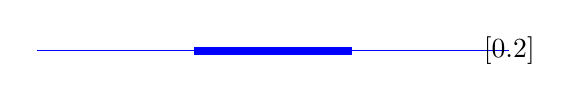
\begin{tikzpicture}
\node at (0,0)[rotate=0, opacity=0.2](s1){};
\draw[draw=blue](s1.center)--++(2cm,0)node(newcoord){};
\node at (newcoord)[rotate=0, opacity=0.2](s2){};
\draw[draw=blue, line width=3pt](s2.center)--++(2cm,0cm)node(newcoord){};
\node at (newcoord)[rotate=-0, opacity=0.2](s3){};
\draw[draw=blue](s3.center)--++(2cm,0cm)node(newcoord){};
\node at (newcoord)[rotate=0, opacity=1](s4){\Scratchy[0.2]};
\end{tikzpicture}
\end{center}
\caption{ಲೇಖನಿ ಗಾತ್ರ ಬದಲಾಯಿಸುವುದು}
\label{pen_linewidth}
\end{figure}
ರೇಖೆಯ ಗಾತ್ರವನ್ನು ಸಂಪೂರ್ಣ ಮೌಲ್ಯ ಉಪಯೋಗಿಸಿ ಬದಲಾಯಿಸ ಬೇಕಾದರೆ,  ಹಸಿರು ಬಣ್ಣದ "ಲೇಖನಿ" ಗುಂಪನ್ನು ಒತ್ತಿ ಅದರಲ್ಲಿನ "\_\_ ರಷ್ಟಕ್ಕೆ ಲೇಖನಿ ಗಾತ್ರವನ್ನು ಹೊಂದಿಸು"ಎಂಬ 
ಆಜ್ಞೆಯನ್ನು ಬಳಸಬೇಕು.  ಚಿತ್ರ \ref{pen_linewidth} ರ ಎಡಭಾಗದಲ್ಲಿರುವಂತೆ ಪ್ರೋಗ್ರಾಮ್ಮನ್ನು ಮೂಡಿಸಿ.  "6 ರಷ್ಟಕ್ಕೆ ಲೇಖನಿ ಗಾತ್ರವನ್ನು ಹೊಂದಿಸು" ಮತ್ತು "1 ರಷ್ಟಕ್ಕೆ ಲೇಖನಿ ಗಾತ್ರವನ್ನು ಹೊಂದಿಸು" ಎಂಬ  ಆಜ್ಞೆಗಳು ಈ ಪ್ರೋಗ್ರಾಮಿನಲ್ಲಿ ಏನು ಕೆಲಸ ಮಾಡುತ್ತಿವೆ ಎಂಬುದರ ಬಗ್ಗೆ ಯೋಚಿಸಿ.  ಪ್ರೋಗ್ರಾಂ ಅನ್ನು  ಚಲಾಯಿಸಿ (ವೇದಿಕೆಯ ಮೇಲಿನ ಹಸಿರು ಧ್ವಜವನ್ನು ಒತ್ತಿ).  ಚಿತ್ರ \ref{pen_linewidth}ರ ಕೆಳಭಾಗದಲ್ಲಿ ತೋರಿಸಿರುವಂತೆ, ಸ್ಪ್ರಯ್ಟ್ ಸಣ್ಣ-ದಪ್ಪ-ಸಣ್ಣ ದಂತಿರುವ ರೇಖೆಯನ್ನು ಮೂಡಿಸುತ್ತದೆ.

ಚಿತ್ರ \ref{pen_linewidth}ನ ಬಲಭಾಗದಲ್ಲಿರುವಂತೆ  ಈ ಪ್ರೊಗ್ರಾಂ ಆನ್ನು ಪುಸ್ತಕದಲ್ಲಿ  ಸರಳವಾಗಿ ಬರೆದುಕೊಳ್ಳಬಹುದು.  

\begin{figure}[h]
\begin{center}
\begin{multicols}{2}
\begin{Scratch}[1]
\beginbox{}
\scbox{ಲೇಖನಿಯುಕ್ತ}{pen}
\scbox{\cb[w]{100} ಹೆಜ್ಜೆ ಮುಂದೆ ಹೋಗು}{motion}
\scbox{ರಷ್ಟಕ್ಕೆ ಲೇಖನಿ ಗಾತ್ರವನ್ನು ಬದಲಾಯಿಸು \cb[w]{5}}{pen}
\scbox{\cb[w]{100} ಹೆಜ್ಜೆ ಮುಂದೆ ಹೋಗು}{motion}
\scbox{ರಷ್ಟಕ್ಕೆ ಲೇಖನಿ ಗಾತ್ರವನ್ನು ಬದಲಾಯಿಸು \cb[w]{5}}{pen}
\scbox{\cb[w]{100} ಹೆಜ್ಜೆ ಮುಂದೆ ಹೋಗು}{motion}
\end{Scratch}

\begin{tikzpicture}
\node[doc] (x) (inst1){
ಒತ್ತಿದಾಗ\\
ಲೇಖನಿಯುಕ್ತ\\
100  ಹೆಜ್ಜೆ ಮುಂದೆ ಹೋಗು\\
5 ರಷ್ಟಕ್ಕೆ ಲೇಖನಿ ಗಾತ್ರವನ್ನು ಬದಲಾಯಿಸು\\
100  ಹೆಜ್ಜೆ ಮುಂದೆ ಹೋಗು\\
5 ರಷ್ಟಕ್ಕೆ ಲೇಖನಿ ಗಾತ್ರವನ್ನು ಬದಲಾಯಿಸು\\
100  ಹೆಜ್ಜೆ ಮುಂದೆ ಹೋಗು
};
\end{tikzpicture}

\end{multicols}

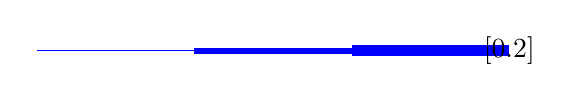
\begin{tikzpicture}
\node at (0,0)[rotate=0, opacity=0.2](s1){};
\draw[draw=blue](s1.center)--++(2cm,0)node(newcoord){};
\node at (newcoord)[rotate=0, opacity=0.2](s2){};
\draw[draw=blue, line width=2pt](s2.center)--++(2cm,0cm)node(newcoord){};
\node at (newcoord)[rotate=-0, opacity=0.2](s3){};
\draw[draw=blue, line width=4pt](s3.center)--++(2cm,0cm)node(newcoord){};
\node at (newcoord)[rotate=0, opacity=1](s4){\Scratchy[0.2]};
\end{tikzpicture}
\end{center}
\caption{ಲೇಖನಿ ಗಾತ್ರವನ್ನು ಸಾಪೇಕ್ಷವಾಗಿ ಬದಲಾಯಿಸುವುದು}
\label{pensize}
\end{figure}

ರೇಖೆಯ ಗಾತ್ರವನ್ನು ಸಾಪೇಕ್ಷ ಮೌಲ್ಯವನ್ನು ಉಪಯೋಗಿಸಿ ಬದಲಾಯಿಸ ಬೇಕಾದರೆ,  "ರಷ್ಟಕ್ಕೆ ಲೇಖನಿ ಗಾತ್ರವನ್ನು ಬದಲಾಯಿಸು \_\_"ಎಂಬ 
ಆಜ್ಞೆಯನ್ನು ಬಳಸಬೇಕು.  ಚಿತ್ರ \ref{pensize} ರ ಎಡಭಾಗದಲ್ಲಿರುವಂತೆ ಪ್ರೋಗ್ರಾಮ್ಮನ್ನು ಮೂಡಿಸಿ.  "ರಷ್ಟಕ್ಕೆ ಲೇಖನಿ ಗಾತ್ರವನ್ನು ಬದಲಾಯಿಸು 5" ಎಂಬ  ಆಜ್ಞೆ ಎರಡು ಬಾರಿ ಬಳಸಿದ್ದೇವೆ.  ಈ ಪ್ರೋಗ್ರಾಮಿನಲ್ಲಿ ಇವು ಏನು ಕೆಲಸ ಮಾಡುತ್ತಿವೆ ಎಂಬುದರ ಬಗ್ಗೆ ಯೋಚಿಸಿ.  

ಪ್ರೋಗ್ರಾಂ ಅನ್ನು  ಚಲಾಯಿಸಿ (ವೇದಿಕೆಯ ಮೇಲಿನ ಹಸಿರು ಧ್ವಜವನ್ನು ಒತ್ತಿ).  ಚಿತ್ರ \ref{pensize}ರ ಕೆಳಭಾಗದಲ್ಲಿ ತೋರಿಸಿರುವಂತೆ, ಸ್ಪ್ರಯ್ಟ್ ಸಣ್ಣ-ದಪ್ಪ-ಅತಿ ದಪ್ಪ ದಂತಿರುವ ರೇಖೆಯನ್ನು ಮೂಡಿಸುತ್ತದೆ.  ಚಿತ್ರ \ref{pensize}ನ ಬಲಭಾಗದಲ್ಲಿರುವಂತೆ  ಈ ಪ್ರೊಗ್ರಾಂ ಆನ್ನು ಪುಸ್ತಕದಲ್ಲಿ  ಸರಳವಾಗಿ ಬರೆದುಕೊಳ್ಳಬಹುದು.  

ಈ ಪ್ರೊಗ್ರಾಮಿನಲ್ಲಿ "ರಷ್ಟಕ್ಕೆ ಲೇಖನಿ ಗಾತ್ರವನ್ನು ಬದಲಾಯಿಸು 5" ಎಂಬ ಎರಡನೇ ಬಾರಿಯ  ಆಜ್ಞೆಯಲ್ಲಿ 5 ಅನ್ನು -5 ಆಗಿ ಬದಲಾಯಿಸಿದರೆ ಏನಾಗುತ್ತದೆ? ಈ ಸವಾಲು ಓದುಗರ ಕುತೂಹಲಕ್ಕೆ. 

\section{ಬಣ್ಣ ಬದಲಾಯಿಸುವುದು}
ರೇಖೆಗಳ ಗಾತ್ರದಂತೆಯೇ ರೇಖೆಗಳ ಬಣ್ಣವನ್ನೂ ಸ್ಕ್ರಾಚ್ನಲ್ಲಿ ಎರಡು ರೀತಿಯಲ್ಲಿ  ಬದಲಾಯಿಸುವ ಅವಕಾಶವಿದೆ - ರೇಖೆಯ ಬಣ್ಣದ ಸಂಪೂರ್ಣ ಮೌಲ್ಯ ಅಥವಾ ಸಾಪೆಕ್ಷ ಮೌಲ್ಯವನ್ನು ನೀಡುವುದರ ಮೂಲಕ.  ಲೇಖನಿ ಗುಂಪಿನಿಂದ "ಲೇಖನಿ ಬಣ್ಣವನ್ನು ಹೊಂದಿಸು" ಎಂಬ ಆಜ್ಞೆಯನ್ನು ಬಳಸಿ ಅದರಲ್ಲಿನ ಸಣ್ಣ ಬಣ್ಣದ ಚೌಕವನ್ನು ಒತ್ತಿದರೆ, ಸ್ಕ್ರಾಚ್ನ ಬಣ್ಣದ ಹಲಗೆ ತೆರೆಯುತ್ತದೆ. ಇದರಿಂದ ನಮಗಿಷ್ಠವಾದ ಬಣ್ಣವನ್ನು ತೆಗೆದುಕೊಳ್ಳಬಹುದು.  ಈ ರೀತಿಯಾಗಿ ರೇಖೆಯ ಬಣ್ಣದ ಸಂಪೂರ್ಣ ಮೌಲ್ಯವನ್ನು ಪ್ರೊಗ್ರಾಮಿನಲ್ಲಿ ಬಳಸಬಹುದು.

\begin{figure}[h]
\begin{center}
\begin{multicols}{2}
\begin{Scratch}[1]
\beginbox{}
\scbox{ಲೇಖನಿಯುಕ್ತ}{pen}
\scbox{\cb[w]{100} ಹೆಜ್ಜೆ ಮುಂದೆ ಹೋಗು}{motion}
\scbox{\sqb{red} ಗೆ ಲೇಖನಿ ಬಣ್ಣವನ್ನು ಹೊಂದಿಸು}{pen}
\scbox{\cb[w]{100} ಹೆಜ್ಜೆ ಮುಂದೆ ಹೋಗು}{motion}
\scbox{\sqb{green} ಗೆ ಲೇಖನಿ ಬಣ್ಣವನ್ನು ಹೊಂದಿಸು}{pen}
\scbox{\cb[w]{100} ಹೆಜ್ಜೆ ಮುಂದೆ ಹೋಗು}{motion}
\end{Scratch}

\begin{tikzpicture}
\node[doc] (x) (inst1){
ಒತ್ತಿದಾಗ\\
ಲೇಖನಿಯುಕ್ತ\\
100  ಹೆಜ್ಜೆ ಮುಂದೆ ಹೋಗು\\
ಕೆಂಪಿಗೆ  ಲೇಖನಿ ಬಣ್ಣವನ್ನು ಹೊಂದಿಸು\\
100  ಹೆಜ್ಜೆ ಮುಂದೆ ಹೋಗು\\
ಹಸಿರಿಗೆ ಲೇಖನಿ ಬಣ್ಣವನ್ನು ಹೊಂದಿಸು\\
100  ಹೆಜ್ಜೆ ಮುಂದೆ ಹೋಗು
};
\end{tikzpicture}

\end{multicols}
\vspace{1cm}
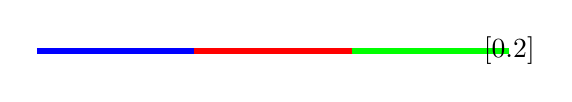
\begin{tikzpicture}
\node at (0,0)[rotate=0, opacity=0.2](s1){};
\draw[draw=blue,line width=2pt](s1.center)--++(2cm,0)node(newcoord){};
\node at (newcoord)[rotate=0, opacity=0.2](s2){};
\draw[draw=red, line width=2pt](s2.center)--++(2cm,0cm)node(newcoord){};
\node at (newcoord)[rotate=-0, opacity=0.2](s3){};
\draw[draw=green,line width=2pt](s3.center)--++(2cm,0cm)node(newcoord){};
\node at (newcoord)[rotate=0, opacity=1](s4){\Scratchy[0.2]};
\end{tikzpicture}
\end{center}
\caption{ಲೇಖನಿ ಬಣ್ಣ ಬದಲಾಯಿಸುವುದು}
\label{pen_color}
\end{figure}
ಉದಾಹರಣೆಗೆ ಚಿತ್ರ \ref{pen_color} ರ ಎಡಭಾಗದಲ್ಲಿರುವಂತೆ ಪ್ರೋಗ್ರಾಮ್ಮನ್ನು ಮೂಡಿಸಿ.  " \_\_ ರಷ್ಟು ಲೇಖನಿ ಬಣ್ಣವನ್ನು ಹೊಂದಿಸು" ಎಂಬ  ಆಜ್ಞೆಗಳು ಈ ಪ್ರೋಗ್ರಾಮಿನಲ್ಲಿ ಹೇಗೆ ಕೆಲಸ ಮಾಡುತ್ತಿವೆ ಎಂಬುದರ ಬಗ್ಗೆ ಯೋಚಿಸಿ.  ಪ್ರೋಗ್ರಾಂ ಅನ್ನು  ಚಲಾಯಿಸಉವುದಕ್ಕೆ ವೇದಿಕೆಯ ಮೇಲಿನ ಹಸಿರು ಧ್ವಜವನ್ನು ಒತ್ತಿ.  ಚಿತ್ರ \ref{pen_color}ರ ಕೆಳಭಾಗದಲ್ಲಿ ತೋರಿಸಿರುವಂತೆ, ಸ್ಪ್ರಯ್ಟ್ ಮೂರು ಬಣ್ಣದ ರೇಖೆಯನ್ನು ಮೂಡಿಸುತ್ತದೆ.  ಚಿತ್ರ \ref{pen_color}ನ ಬಲಭಾಗದಲ್ಲಿರುವಂತೆ  ಈ ಪ್ರೊಗ್ರಾಂ ಆನ್ನು ಪುಸ್ತಕದಲ್ಲಿ  ಸರಳವಾಗಿ ಬರೆದುಕೊಳ್ಳಬಹುದು.  

\begin{figure}[h]
\begin{center}
\begin{multicols}{2}
\begin{Scratch}[1]
\beginbox{}
\scbox{ಲೇಖನಿಯುಕ್ತ}{pen}
\scbox{\cb[w]{100} ಹೆಜ್ಜೆ ಮುಂದೆ ಹೋಗು}{motion}
\scbox{ರಷ್ಟು ಲೇಖನಿ ಬಣ್ಣ ಬದಲಾಯಿಸು \cb[w]{80}}{pen}
\scbox{\cb[w]{100} ಹೆಜ್ಜೆ ಮುಂದೆ ಹೋಗು}{motion}
\scbox{ರಷ್ಟು ಲೇಖನಿ ಬಣ್ಣ ಬದಲಾಯಿಸು \cb[w]{80}}{pen}
\scbox{\cb[w]{100} ಹೆಜ್ಜೆ ಮುಂದೆ ಹೋಗು}{motion}
\end{Scratch}

\begin{tikzpicture}
\node[doc] (x) (inst1){
ಒತ್ತಿದಾಗ\\
ಲೇಖನಿಯುಕ್ತ\\
100  ಹೆಜ್ಜೆ ಮುಂದೆ ಹೋಗು\\
80 ರಷ್ಟು ಲೇಖನಿ ಬಣ್ಣ ಬದಲಾಯಿಸು\\
100  ಹೆಜ್ಜೆ ಮುಂದೆ ಹೋಗು\\
80 ರಷ್ಟು ಲೇಖನಿ ಬಣ್ಣ ಬದಲಾಯಿಸು\\
100  ಹೆಜ್ಜೆ ಮುಂದೆ ಹೋಗು
};
\end{tikzpicture}

\end{multicols}
\vspace{1cm}
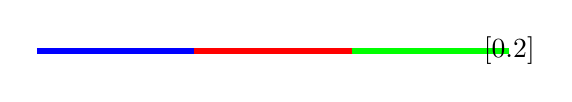
\begin{tikzpicture}
\node at (0,0)[rotate=0, opacity=0.2](s1){};
\draw[draw=blue,line width=2pt](s1.center)--++(2cm,0)node(newcoord){};
\node at (newcoord)[rotate=0, opacity=0.2](s2){};
\draw[draw=red, line width=2pt](s2.center)--++(2cm,0cm)node(newcoord){};
\node at (newcoord)[rotate=-0, opacity=0.2](s3){};
\draw[draw=green,line width=2pt](s3.center)--++(2cm,0cm)node(newcoord){};
\node at (newcoord)[rotate=0, opacity=1](s4){\Scratchy[0.2]};
\end{tikzpicture}
\end{center}
\caption{ಲೇಖನಿ ಬಣ್ಣವನ್ನು ಸಾಪೇಕ್ಷವಾಗಿ ಬದಲಾಯಿಸುವುದು}
\label{pen_color_rel}
\end{figure}
ಸಾಪೇಕ್ಷ ಮೌಲ್ಯವನ್ನು ಉಪಯೋಗಿಸಿ ರೇಖೆಯ ಬಣ್ಣವನ್ನು ಬದಲಾಯಿಸ ಬೇಕಾದರೆ,  "ರಷ್ಟಕ್ಕೆ ಲೇಖನಿ ಬಣ್ನವನ್ನು ಬದಲಾಯಿಸು \_\_"ಎಂಬ ಆಜ್ಞೆಯನ್ನು ಬಳಸಬೇಕು.  

ಚಿತ್ರ \ref{pen_color_rel} ರ ಎಡಭಾಗದಲ್ಲಿರುವಂತೆ ಪ್ರೋಗ್ರಾಮ್ಮನ್ನು ಮೂಡಿಸಿ.  "ರಷ್ಟಕ್ಕೆ ಲೇಖನಿ ಬಣ್ಣವನ್ನು ಬದಲಾಯಿಸು 80" ಎಂಬ  ಆಜ್ಞೆ ಎರಡು ಬಾರಿ ಬಳಸಿದ್ದೇವೆ.  ಈ ಪ್ರೋಗ್ರಾಮಿನಲ್ಲಿ ಇವುಗಳ  ಪರಿಣಮವೇನು ಎಂಬುದರ ಬಗ್ಗೆ ಯೋಚಿಸಿ. ಪ್ರೋಗ್ರಾಂ ಅನ್ನು ವೇದಿಕೆಯ ಮೇಲಿನ ಹಸಿರು ಧ್ವಜವನ್ನು ಒತ್ತುವುದರ ಮೂಲಕ ಚಲಾಯಿಸಿ ನೋಡಿ.  ಚಿತ್ರ \ref{pen_color_rel}ರ ಕೆಳಭಾಗದಲ್ಲಿ ತೋರಿಸಿರುವಂತೆ, ಸ್ಪ್ರಯ್ಟ್ ಮೂರು ಬಣ್ಣದ ರೇಖೆಯನ್ನು ಮೂಡಿಸುತ್ತದೆ.  ಚಿತ್ರ \ref{pen_color_rel}ನ ಬಲಭಾಗದಲ್ಲಿರುವಂತೆ  ಈ ಪ್ರೊಗ್ರಾಮನ್ನು  ಪುಸ್ತಕದಲ್ಲಿ  ಸರಳವಾಗಿ ಬರೆದುಕೊಳ್ಳಬಹುದು.  

ರೇಖೆಯ ಬಣ್ಣದ ಛಾಯೆಯನ್ನೂ ಸಂಪೂರ್ಣ ಅಥವಾ ಸಾಪೇಕ್ಷ ಮೌಲ್ಯವನ್ನು ಉಪಯೋಗಿಸಿ ಬದಲಾಯಿಸಬಹುದು.  " \_\_ ರಷ್ಟಕ್ಕೆ ಲೇಖನಿ ನೆರಳನ್ನು ಹೊಂದಿಸು" ಅಥವಾ "ರಷ್ಟಕ್ಕೆ ಲೇಖನಿ ನೆರಳನ್ನು ಬದಲಾಯಿಸು \_\_" ಎಂಬ ಆಜ್ಞೆಗಳನ್ನು ಬಳಸಿದರೆ ರೇಖೆಯ ಬಣ್ಣದ ಛಾಯೆ ಬದಲಾಗುತ್ತದೆ.  "ಲೇಖನಿ ಬಣ್ಣವನ್ನು ಹೊಂದಿಸು" ಎಂಬ ಆಜ್ಞೆಯನ್ನು ಬಳಸಿ ಅದರಲ್ಲಿನ ಸಣ್ಣ ಬಣ್ಣದ ಚೌಕವನ್ನು ಒತ್ತಿ, ಬಣ್ಣದ ಹಲಗೆಯಿಂದ ನಮಗಿಷ್ಠವಾದ ಬಣ್ಣವನ್ನು ತೆಗೆದುಕೊಳ್ಳಬಹುದಾದರೂ ಸಂಪೂರ್ಣ ಮೌಲ್ಯ ಉಪಯೋಗಿಸಿ ರೇಖೆಯ ಬಣ್ಣಾ ಬದಲಾಯಿಸುವುದಕ್ಕೆ ಮತ್ತೊಂದು ಮಾರ್ಗ ಇದೆ.  "\_\_ ಗೆ ಲೇಖನಿ ಬಣ್ಣವನ್ನು ಹೊಂದಿಸು" ಎಂಬ ಆಜ್ಞೆಯನ್ನು ಪ್ರೋಗ್ರಾಮಿನಲ್ಲಿ ಬಳಾಸಿ ಆಜ್ಞೆಯಲ್ಲಿನ ಸಂಖ್ಯೆಯನ್ನು ಬದಲಾಯಿಸಿ ನೋಡಿ. 

\section{ಅಭ್ಯಾಸ }
ಇನ್ನು ಓದುಗರ ಸಮಯ ಮತ್ತು ಆಸಕ್ತಿಗೆ ತಕ್ಕಂತೆ ಕೆಳಗಿನ ಪ್ರೋಗ್ರಾಂಗಳನ್ನು ಅಭ್ಯಾಸಕ್ಕಾಗಿ ಮಾಡಬಹುದು.

\begin{figure}[h]
1. ಸ್ಪ್ರಯ್ಟ್ ಆಯತವನ್ನು ಬಿಡಿಸುವಂತೆ ಪ್ರೊಗ್ರಾಂ ಮೊದಲು ಪುಸ್ತಕದಲ್ಲಿ ಪ್ರಯತ್ನಿಸಿ, ನಂತರ ಸ್ಕ್ರಾಚ್ನಲ್ಲಿ ಮಾಡಿ. 
\begin{center}
\begin{tikzpicture}
\node at (0,0)[draw=blue,  rectangle, minimum width = 4cm, minimum height=2cm](s1){};
\node at (s1.north east)[rotate=0, opacity=1](s2){\Scratchy[0.2]};
\end{tikzpicture}
\end{center}
\caption{ಸ್ಪ್ರಯ್ಟ್ ಇಂದ  ಆಯತವನ್ನು ಬಿಡಿಸುವುದು}
\label{pen_program1}
\end{figure}

\begin{figure}[h]
2. ಸ್ಪ್ರಯ್ಟ್ ಕೇಂದ್ರೀಕೃತ ಚೌಕವನ್ನು ಬಿಡಿಸುವಂತೆ ಪ್ರೊಗ್ರಾಂ ಬರೆಯಿರಿ. ಮೊದಲು ಪುಸ್ತಕದಲ್ಲಿ ಪ್ರಯತ್ನಿಸಿ ನಂತರ ಸ್ಕ್ರಾಚ್ನಲ್ಲಿ ಮಾಡಿ ನೋಡಿ. 
\begin{center}
\begin{tikzpicture}
\node at (0,0)[draw=blue,  rectangle, minimum width = 3cm, minimum height=3cm](s1){};
\node at (s1.north east)[rotate=0, opacity=1](s2){\Scratchy[0.2]};
\node at (s1.center)[anchor=center, draw=blue,  rectangle, minimum width = 1.5cm, minimum height=1.5cm](s3){};
\end{tikzpicture}
\end{center}
\caption{ಸ್ಪ್ರಯ್ಟ್ ಇಂದ ಕೇಂದ್ರೀಕೃತ ಚೌಕವನ್ನು ಬಿಡಿಸುವುದು}
\label{pen_program2}
\end{figure}


\begin{figure}[h]
3. ಸ್ಪ್ರಯ್ಟ್ ಇಂದ ಮುರಿದ ರೇಖೆಗಳ ಚೌಕವನ್ನು ಬಿಡಿಸುವಂತೆ ಪ್ರೊಗ್ರಾಂ ಬರೆಯಿರಿ. \begin{center}
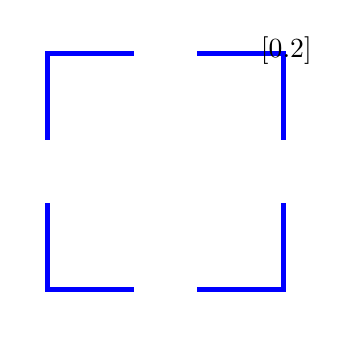
\begin{tikzpicture}
\node at (0,0)[draw=blue,  line width = 2pt, rectangle, minimum width = 3cm, minimum height=3cm](s1){};
\node at (s1.center)[anchor=center, draw=none,  fill=white, rectangle, minimum width = 0.8cm, minimum height=3.5cm](s2){};
\node at (s1.center)[anchor=center, draw=none,  fill=white, rectangle, minimum width = 3.5cm, minimum height=0.8cm](s3){};
\node at (s1.north east)[rotate=0, opacity=1](s4){\Scratchy[0.2]};
\end{tikzpicture}
\end{center}
\caption{ಸ್ಪ್ರಯ್ಟ್ ಮುರಿದ-ರೇಖೆಗಳ ಚೌಕವನ್ನು ಬಿಡಿಸುವುದು}
\label{pen_program3}
\end{figure}

\begin{figure}[h]
4. ಸ್ಪ್ರಯ್ಟ್ ವಿವಿಧ ಗಾತ್ರದ ರೇಖೆಗಳ ಚೌಕವನ್ನು ಬಿಡಿಸುವಂತೆ ಪ್ರೊಗ್ರಾಂ ಬರೆಯಿರಿ. 
\begin{center}
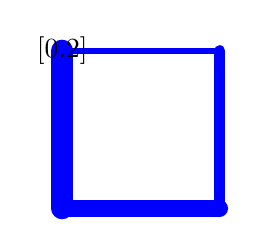
\begin{tikzpicture}
\draw[draw=blue, line width=2pt,line cap=round] (0,0)--++(2cm,0) coordinate (a);
\draw[draw=blue, line width=4pt,line cap=round] (a)--++(0,-2cm) coordinate (a);
\draw[draw=blue, line width=6pt,line cap=round] (a)--++(-2cm,0) coordinate (a);
\draw[draw=blue, line width=8pt,line cap=round] (a)--++(0,2cm) coordinate (a);
\node at (a)[rotate=0, opacity=1, anchor=center](s4){\Scratchy[0.2]};
\end{tikzpicture}
\end{center}
\caption{ಸ್ಪ್ರಯ್ಟ್ ವಿವಿಧ ಗಾತ್ರದ ರೇಖೆಗಳಿಂದ ಚೌಕವನ್ನು ಬಿಡಿಸುವುದು}
\label{pen_program4}
\end{figure}

\begin{figure}[h]
5.ಸ್ಪ್ರಯ್ಟ್ ವಿವಿಧ ಬಣ್ಣದ ರೇಖೆಗಳ ಚೌಕವನ್ನು ಬಿಡಿಸುವಂತೆ ಪ್ರೋಗ್ರಾಂ ಬರೆಯಿರಿ. \begin{center}
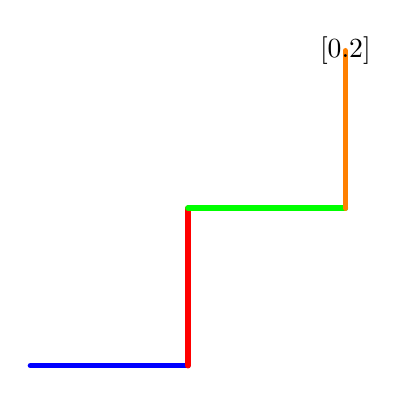
\begin{tikzpicture}
\draw[draw=blue, line width=2pt,line cap=round] (0,0)--++(2cm,0) coordinate (a);
\draw[draw=red, line width=2pt,line cap=round] (a)--++(0,2cm) coordinate (a);
\draw[draw=green, line width=2pt,line cap=round] (a)--++(2cm,0) coordinate (a);
\draw[draw=orange, line width=2pt,line cap=round] (a)--++(0,2cm) coordinate (a);
\node at (a)[rotate=0, opacity=1, anchor=center](s4){\Scratchy[0.2]};
\end{tikzpicture}
\end{center}
\caption{ಸ್ಪ್ರಯ್ಟ್ ವಿವಿಧ ಬಣ್ಣದ ರೇಖೆಗಳಿಂದ ಚೌಕವನ್ನು ಬಿಡಿಸುವುದು}
\label{pen_program5}
\end{figure}

\begin{figure}[h]
6. ಸ್ಪ್ರಯ್ಟ್ ನಿಂದ ಒಂದು ಜಟಿಲವನ್ನು ತಯಾರಿಸಿರಿ
\begin{center}
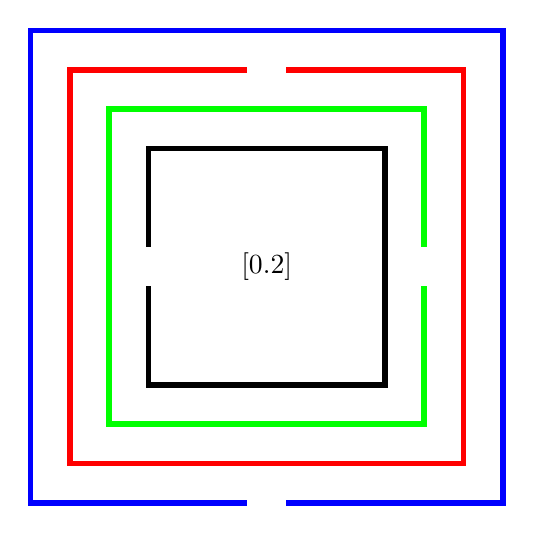
\begin{tikzpicture}
\node at (0,0)[draw=blue,  rectangle, line width=2pt, minimum width = 6cm, minimum height=6cm](s1){};
\node at (s1.center)[rotate=0, opacity=1](s2){\Scratchy[0.2]};
\node at (s1.center)[anchor=center, draw=red,   line width=2pt, rectangle, minimum width = 5cm, minimum height=5cm](s3){};
\node at (s3.center)[anchor=center, draw=green,   line width=2pt, rectangle, minimum width = 4cm, minimum height=4cm](s4){};
\node at (s4.center)[anchor=center, draw=black,   line width=2pt, rectangle, minimum width = 3cm, minimum height=3cm](s5){};

\node at (s1.south)[anchor=center, draw=none, fill=white,  rectangle, minimum width = 0.5cm, minimum height=0.2cm](o1){};
\node at (s3.north)[anchor=center, draw=none, fill=white,  rectangle, minimum width = 0.5cm, minimum height=0.2cm](o2){};
\node at (s4.east)[anchor=center, draw=none, fill=white,  rectangle, minimum width = 0.2cm, minimum height=0.5cm](o3){};
\node at (s5.west)[anchor=center, draw=none, fill=white,  rectangle, minimum width = 0.2cm, minimum height=0.5cm](o4){};
\end{tikzpicture}
\end{center}
\caption{ಸ್ಪ್ರಯ್ಟ್ ಅನ್ನು ಒಂದು ಜಟಿಲದಿಂದ ಹೊರತರುವುದು}
\label{pen_program5}
\end{figure}
